% experiments.tex -- Section 4: Main Results
% Experiment IDs (provenance):
%   Baseline 44.8%:              eval_stage1_only
%   ACIS k=0.5 zero-mask:       eval_stage1only_object_v2_fixed
%   ACIS k=0.7 zero-mask:       eval_k07_zero_mask
%   ACIS k=0.9 zero-mask:       eval_stage1only_k09
%   Random k=0.5:               eval_random_prune_k05
%   True removal k=0.5:         eval_true_removal_k05
%   Merge k=0.5:                eval_merge_k05
%   Spatial suite:              eval_spatial_prune_k05 (baseline 51.8%)
%   Goal suite:                 eval_goal_prune_k05 (baseline 63%)

\section{Main Results}
\label{sec:results}

Vision token pruning in Vision Transformers (ViTs) is widely regarded as a reliable efficiency technique.
DynamicViT~\cite{rao2021dynamicvit} removes 30\%--50\% of tokens with less than 0.5\% accuracy loss on ImageNet, and Token Merging (ToMe)~\cite{bolya2023tome} merges up to 40\% of tokens while retaining over 99\% of classification accuracy.
EViT~\cite{liang2022evit} similarly discards 50\% of inattentive tokens with negligible degradation.
These results have motivated recent proposals to apply similar strategies to Vision-Language-Action (VLA) models for real-time robotic control~\cite{xu2025vlacache,cheng2026vlaiap}.
Our experiments test whether this transfer holds: we apply six pruning configurations to a VLA policy and evaluate closed-loop Success Rate (SR) on the LIBERO benchmark~\cite{liu2023libero}.
The result is unambiguous.
Every configuration produces 0\% SR, a complete collapse we term the \emph{cliff edge}.

\begin{table}[t]
\centering
\caption{Ablation matrix across scoring functions, retention ratios, and pruning mechanisms. All six pruning conditions produce 0\% SR. The baseline runs the same checkpoint with pruning disabled (bypass mode). Wilson 95\% confidence intervals (CI) are computed over independent episodes. Experiment IDs are listed for reproducibility.}
\label{tab:ablation_matrix}
\small
\begin{tabular}{@{}llccrrc@{}}
\toprule
Method & Scoring & $k$ & Mechanism & SR (\%) & Episodes & Wilson 95\% CI \\
\midrule
\textbf{Baseline} & \textbf{--} & \textbf{1.0} & \textbf{--} & \textbf{44.8} & \textbf{500} & \textbf{[40.5, 49.2]} \\
\midrule
ACIS & Learned & 0.5 & Zero-mask & 0.0 & 300+ & [0.0, 1.26] \\
ACIS & Learned & 0.7 & Zero-mask & 0.0 & 500 & [0.0, 0.76] \\
ACIS & Learned & 0.9 & Zero-mask & 0.0 & 500 & [0.0, 0.76] \\
Random & Random & 0.5 & Zero-mask & 0.0 & 500 & [0.0, 0.76] \\
ACIS & Learned & 0.5 & True removal & 0.0 & 500 & [0.0, 0.80] \\
ACIS & Learned & 0.5 & Merge & 0.0 & 500 & [0.0, 0.76] \\
\bottomrule
\end{tabular}
\end{table}

Table~\ref{tab:ablation_matrix} presents the full ablation matrix.
We systematically vary three axes: (1)~the scoring function that selects which tokens to prune, (2)~the retention ratio $k$ that controls how many tokens survive, and (3)~the mechanism by which pruned tokens are handled.
The baseline achieves 44.8\% SR across 500 episodes using the identical model checkpoint with pruning disabled.
All six pruning conditions collapse to 0\% SR.

\paragraph{Scoring axis.}
If the failure were caused by a poor scoring function that discards the wrong tokens, replacing the learned Attention-weighted Cumulative Importance Score (ACIS) scorer with uniform random selection should produce a different outcome.
It does not: random pruning at $k{=}0.5$ also yields 0\% SR over 500 episodes (Table~\ref{tab:ablation_matrix}, row~5).
The cliff edge is therefore not a scoring quality problem.
No matter which tokens are selected for removal, the policy collapses.

\paragraph{Ratio axis.}
If the failure were caused by removing too many tokens, retaining 90\% of tokens ($k{=}0.9$, removing only 10\%) should preserve most task-relevant information.
Yet $k{=}0.9$ also produces 0\% SR (Table~\ref{tab:ablation_matrix}, row~3).
This rules out the hypothesis that a gentler pruning ratio would recover graceful degradation.
The transition from functional to non-functional is binary, not gradual.

\paragraph{Mechanism axis.}
Three distinct mechanisms for handling pruned tokens produce identical failure.
Zero-masking replaces pruned token embeddings with zeros, which could inject out-of-distribution (OOD) activation patterns.
True removal eliminates the tokens entirely, changing the sequence length but avoiding OOD injection.
Token merging (following ToMe~\cite{bolya2023tome}) combines pruned tokens with their nearest neighbors, preserving sequence length and total information.
All three mechanisms yield 0\% SR (Table~\ref{tab:ablation_matrix}, rows~2, 6, 7).
The collapse is therefore not caused by OOD activations from a particular masking strategy; it is a property of any alteration to the vision token sequence.

\begin{figure}[t]
\centering
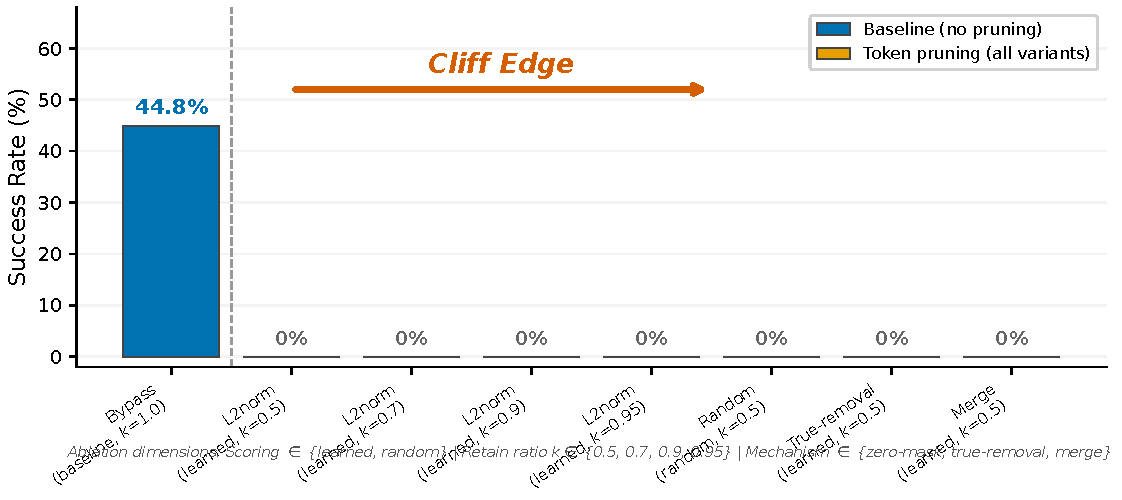
\includegraphics[width=\linewidth]{figures/paper/fig_cliff_edge.pdf}
\caption{The cliff edge in VLA token pruning. While ViT pruning methods retain $>$99\% accuracy on classification benchmarks even at aggressive retention ratios~\cite{rao2021dynamicvit,bolya2023tome,liang2022evit}, applying any form of token reduction to a VLA policy causes immediate collapse to 0\% SR across all LIBERO suites. The transition from functional to non-functional is binary, with no intermediate degradation regime.}
\label{fig:cliff_edge}
\end{figure}

\paragraph{Cross-suite confirmation.}
To verify that the cliff edge is not an artifact of a single task distribution, we evaluate ACIS pruning at $k{=}0.5$ across three LIBERO suites with distinct characteristics.
On LIBERO-Object (object manipulation), SR drops from 44.8\% to 0\%.
On LIBERO-Spatial (spatial reasoning), SR drops from 51.8\% to 0\%.
On LIBERO-Goal (goal-conditioned tasks), SR drops from 63.0\% to 0\%.
The cliff edge is consistent across all three suites, and the absolute SR gap is largest for the suite where the baseline performs best (63 percentage points for Goal).
Figure~\ref{fig:cliff_edge} visualizes this collapse pattern.
These results establish that the cliff edge is method-agnostic: it persists regardless of which tokens are pruned, how aggressively they are pruned, and how the pruning is implemented.
The phenomenon is not a failure of any particular pruning algorithm but a structural property of how VLA policies consume vision tokens during closed-loop control.
